\documentclass[twoside,11pt]{article}

% +
%  Name:
%     sun230.tex

%  Purpose:
%     SUN documentation for ORAC-DR overview (SUN/230)

%  Authors:
%     Frossie Economou (JACH)
%     Tim Jenness (JACH)

%  Copyright:
%     Copyright (C) 1997-2003 Particle Physics and Astronomy
%     Research Council. All Rights Reserved.

%  Notes:
%     The final SUN is generated automatically from POD. Once the
%     latex is generated the following changes are required:
%     - Replace ORAC-DR with \oracdr\
%     - Remove any junk from the start and end of each pod section.
%       Usually involves removing everything up to and including the
%       DESCRIPTION section declaration, leaving the description in place
%       as a section introduction. Remove COPYRIGHT, AUTHOR and REVISION
%       sections.
%     - Remove % from end of pod2latex generated \item commands (and
%       \index commands) since they are not needed
%       and they ruin the star2html conversion.
%     - Usually replace 'this document' with 'this section'
%     - Add xlabels to all sections/subsections
%     - References to CGS4DR should be replaced with \cgsdr\
%     - References to GAIA should be replaced with \gaia\
%     - References to GWM should be replaced with \gwm\
%     - References to Kappa should be replaced with \Kappa\
%     - References to KAPVIEW should be replaced with \kapview\
%     - References to EXTRACTOR should be replaced with \extractor\
%     - Replace P4 with \textsc{p4}
%     - Replace (C) with \copyright
%     - Replace SUN/231 and SUN/232 references with real xrefs

%  History:
%     $Log$
%     Revision 1.10  2004/05/27 20:10:09  bradc
%     updates for ORAC-DR v4.1-0
%
%     Revision 1.9  2003/06/13 03:58:01  timj
%     Update for V4.0 release.
%
%     Revision 1.8  2002/09/16 04:29:42  timj
%     - fix up header, abstract and release notes for V3.1-3
%
%     Revision 1.7  2001/11/19 04:11:16  timj
%     Add release notes
%
%     Revision 1.6  2001/11/17 01:28:43  timj
%     Prep version 3.0 starlink release
%
%     Revision 1.5  2001/04/11 03:52:26  timj
%     Add stardoccopyright
%
%     Revision 1.4  2001/04/10 21:52:19  timj
%     - update doc number
%     - Add Alasdair Allan
%     - Add CGS4
%
%     Revision 1.3  2000/02/09 20:19:41  timj
%     Correct stardocnumber to .1 rather than .0
%
%     Revision 1.2  2000/02/08 04:41:10  timj
%     Fixes to documentation required by Starlink for release of V1.0-0
%
%     Revision 1.1.1.1  2000/02/03 09:44:59  timj
%     first starlink docs
%

%  Revision:
%     $Id$

% -

% ? Specify used packages
\usepackage{graphicx}        %  Use this one for final production.
\usepackage{times}
% \usepackage[draft]{graphicx} %  Use this one for drafting.
% ? End of specify used packages

\pagestyle{myheadings}

% -----------------------------------------------------------------------------
% ? Document identification
% Fixed part
\newcommand{\stardoccategory}  {Starlink User Note}
\newcommand{\stardocinitials}  {SUN}
\newcommand{\stardocsource}    {sun\stardocnumber}

% Variable part - replace [xxx] as appropriate.
\newcommand{\stardocnumber}    {230.6}
\newcommand{\stardocauthors}   {Frossie Economou, Tim Jenness,\\
Malcolm Currie, Andy Adamson, Alasdair Allan, Brad Cavanagh\\
Joint Astronomy Centre, Hilo, Hawaii}
\newcommand{\stardoccopyright} {Copyright \copyright\ 1997-2004 Particle Physics and Astronomy Research Council}
\newcommand{\stardocdate}      {June 2004}
\newcommand{\stardoctitle}     {ORAC-DR: Overview and General Introduction}
\newcommand{\stardocversion}   {4.1-0}
\newcommand{\stardocmanual}    {}


\newcommand{\stardocabstract} {\textsc{orac-dr} is a general purpose automatic
  data reduction pipeline environment. It currently supports data reduction
  for the United Kingdom Infrared Telescope (UKIRT) instruments UFTI, IRCAM,
  UIST  and CGS4, for the James Clerk Maxwell Telescope (JCMT) instrument
  SCUBA, for the William Herschel Telescope (WHT) instrument INGRID, for the
  European Southern Observatory (ESO) instrument ISAAC and
  for the Anglo-Australian Telescope (AAT) instrument IRIS-2. This document
  describes the general pipeline environment. For specific information on how
  to reduce the data for a particular instrument, please consult the
  appropriate \textsc{orac-dr} instrument guide.}

% ? End of document identification
% -----------------------------------------------------------------------------

% +
%  Name:
%     sun.tex
%
%  Purpose:
%     Template for Starlink User Note (SUN) documents.
%     Refer to SUN/199
%
%  Authors:
%     AJC: A.J.Chipperfield (Starlink, RAL)
%     BLY: M.J.Bly (Starlink, RAL)
%     PWD: Peter W. Draper (Starlink, Durham University)
%
%  History:
%     17-JAN-1996 (AJC):
%        Original with hypertext macros, based on MDL plain originals.
%     16-JUN-1997 (BLY):
%        Adapted for LaTeX2e.
%        Added picture commands.
%     13-AUG-1998 (PWD):
%        Converted for use with LaTeX2HTML version 98.2 and
%        Star2HTML version 1.3.
%     {Add further history here}
%
% -

\newcommand{\stardocname}{\stardocinitials /\stardocnumber}
\markboth{\stardocname}{\stardocname}
\setlength{\textwidth}{160mm}
\setlength{\textheight}{230mm}
\setlength{\topmargin}{-2mm}
\setlength{\oddsidemargin}{0mm}
\setlength{\evensidemargin}{0mm}
\setlength{\parindent}{0mm}
\setlength{\parskip}{\medskipamount}
\setlength{\unitlength}{1mm}

% -----------------------------------------------------------------------------
%  Hypertext definitions.
%  ======================
%  These are used by the LaTeX2HTML translator in conjunction with star2html.

%  Comment.sty: version 2.0, 19 June 1992
%  Selectively in/exclude pieces of text.
%
%  Author
%    Victor Eijkhout                                      <eijkhout@cs.utk.edu>
%    Department of Computer Science
%    University Tennessee at Knoxville
%    104 Ayres Hall
%    Knoxville, TN 37996
%    USA

%  Do not remove the %begin{latexonly} and %end{latexonly} lines (used by
%  LaTeX2HTML to signify text it shouldn't process).
%begin{latexonly}
\makeatletter
\def\makeinnocent#1{\catcode`#1=12 }
\def\csarg#1#2{\expandafter#1\csname#2\endcsname}

\def\ThrowAwayComment#1{\begingroup
    \def\CurrentComment{#1}%
    \let\do\makeinnocent \dospecials
    \makeinnocent\^^L% and whatever other special cases
    \endlinechar`\^^M \catcode`\^^M=12 \xComment}
{\catcode`\^^M=12 \endlinechar=-1 %
 \gdef\xComment#1^^M{\def\test{#1}
      \csarg\ifx{PlainEnd\CurrentComment Test}\test
          \let\html@next\endgroup
      \else \csarg\ifx{LaLaEnd\CurrentComment Test}\test
            \edef\html@next{\endgroup\noexpand\end{\CurrentComment}}
      \else \let\html@next\xComment
      \fi \fi \html@next}
}
\makeatother

\def\includecomment
 #1{\expandafter\def\csname#1\endcsname{}%
    \expandafter\def\csname end#1\endcsname{}}
\def\excludecomment
 #1{\expandafter\def\csname#1\endcsname{\ThrowAwayComment{#1}}%
    {\escapechar=-1\relax
     \csarg\xdef{PlainEnd#1Test}{\string\\end#1}%
     \csarg\xdef{LaLaEnd#1Test}{\string\\end\string\{#1\string\}}%
    }}

%  Define environments that ignore their contents.
\excludecomment{comment}
\excludecomment{rawhtml}
\excludecomment{htmlonly}

%  Hypertext commands etc. This is a condensed version of the html.sty
%  file supplied with LaTeX2HTML by: Nikos Drakos <nikos@cbl.leeds.ac.uk> &
%  Jelle van Zeijl <jvzeijl@isou17.estec.esa.nl>. The LaTeX2HTML documentation
%  should be consulted about all commands (and the environments defined above)
%  except \xref and \xlabel which are Starlink specific.

\newcommand{\htmladdnormallinkfoot}[2]{#1\footnote{#2}}
\newcommand{\htmladdnormallink}[2]{#1}
\newcommand{\htmladdimg}[1]{}
\newcommand{\hyperref}[4]{#2\ref{#4}#3}
\newcommand{\htmlref}[2]{#1}
\newcommand{\htmlimage}[1]{}
\newcommand{\htmladdtonavigation}[1]{}

\newenvironment{latexonly}{}{}
\newcommand{\latex}[1]{#1}
\newcommand{\html}[1]{}
\newcommand{\latexhtml}[2]{#1}
\newcommand{\HTMLcode}[2][]{}

%  Starlink cross-references and labels.
\newcommand{\xref}[3]{#1}
\newcommand{\xlabel}[1]{}

%  LaTeX2HTML symbol.
\newcommand{\latextohtml}{\LaTeX2\texttt{HTML}}

%  Define command to re-centre underscore for Latex and leave as normal
%  for HTML (severe problems with \_ in tabbing environments and \_\_
%  generally otherwise).
\renewcommand{\_}{\texttt{\symbol{95}}}

% -----------------------------------------------------------------------------
%  Debugging.
%  =========
%  Remove % on the following to debug links in the HTML version using Latex.

% \newcommand{\hotlink}[2]{\fbox{\begin{tabular}[t]{@{}c@{}}#1\\\hline{\footnotesize #2}\end{tabular}}}
% \renewcommand{\htmladdnormallinkfoot}[2]{\hotlink{#1}{#2}}
% \renewcommand{\htmladdnormallink}[2]{\hotlink{#1}{#2}}
% \renewcommand{\hyperref}[4]{\hotlink{#1}{\S\ref{#4}}}
% \renewcommand{\htmlref}[2]{\hotlink{#1}{\S\ref{#2}}}
% \renewcommand{\xref}[3]{\hotlink{#1}{#2 -- #3}}
%end{latexonly}
% -----------------------------------------------------------------------------
% ? Document specific \newcommand or \newenvironment commands.

\def\C++{{\rm C\kern-.05em\raise.3ex\hbox{\footnotesize ++}}}
\newcommand{\underscore}{\_}
\newcommand{\oracdr}{\textsc{orac-dr}}

% For HTML redefine hfil since latex2html does not understand it
\html{\renewcommand{\hfil}{ }}

\newcommand{\recipe}[1]{{\small\textsf{#1}}}
\newcommand{\primitive}[1]{{\small\texttt{#1}}}

\newcommand{\Kappa}{\xref{{\textsc{Kappa}}}{sun95}{}}
\newcommand{\kapview}{\textsc{kapview}}
\newcommand{\gaia}{\xref{{\textsc{Gaia}}}{sun214}{}}
\newcommand{\cgsdr}{\xref{{\textsc{cgs4dr}}}{sun27}{}}
\newcommand{\gwm}{\xref{\textsc{gwm}}{sun219}{}}
\newcommand{\extractor}{\xref{\textsc{extractor}}{sun226}{}}

% ? End of document specific commands
% -----------------------------------------------------------------------------
%  Title Page.
%  ===========
\renewcommand{\thepage}{\roman{page}}
\begin{document}
\thispagestyle{empty}

%  Latex document header.
%  ======================
\begin{latexonly}
   CCLRC / \textsc{Rutherford Appleton Laboratory} \hfill \textbf{\stardocname}\\
   {\large Particle Physics \& Astronomy Research Council}\\
   {\large Starlink Project\\}
   {\large \stardoccategory\ \stardocnumber}
   \begin{flushright}
   \stardocauthors\\
   \stardocdate
   \end{flushright}
   \vspace{-4mm}
   \rule{\textwidth}{0.5mm}
   \vspace{5mm}
   \begin{center}
   {\Huge\textbf{\stardoctitle \\ [2.5ex]}}
   {\LARGE\textbf{\stardocversion \\ [4ex]}}
   {\Huge\textbf{\stardocmanual}}
   \end{center}
   \vspace{5mm}

% ? Add picture here if required for the LaTeX version.
%   e.g. \includegraphics[scale=0.3]{filename.ps}
\begin{center}

\includegraphics[width=1.0in]{sun230_logo.eps}
\end{center}
% ? End of picture

% ? Heading for abstract if used.
   \vspace{10mm}
   \begin{center}
      {\Large\textbf{Abstract}}
   \end{center}
% ? End of heading for abstract.
\end{latexonly}

%  HTML documentation header.
%  ==========================
\begin{htmlonly}
   \xlabel{}
   \begin{rawhtml} <H1> \end{rawhtml}
      \stardoctitle\\
      \stardocversion\\
      \stardocmanual
   \begin{rawhtml} </H1> <HR> \end{rawhtml}

% ? Add picture here if required for the hypertext version.
%   e.g. \includegraphics[scale=0.7]{filename.ps}

\includegraphics[width=1.0in]{sun230_logo.eps}
% ? End of picture

   \begin{rawhtml} <P> <I> \end{rawhtml}
   \stardoccategory\ \stardocnumber \\
   \stardocauthors \\
   \stardocdate
   \begin{rawhtml} </I> </P> <H3> \end{rawhtml}
      \htmladdnormallink{CCLRC / Rutherford Appleton Laboratory}
                        {http://www.cclrc.ac.uk} \\
      \htmladdnormallink{Particle Physics \& Astronomy Research Council}
                        {http://www.pparc.ac.uk} \\
   \begin{rawhtml} </H3> <H2> \end{rawhtml}
      \htmladdnormallink{Starlink Project}{http://www.starlink.rl.ac.uk/}
   \begin{rawhtml} </H2> \end{rawhtml}
   \htmladdnormallink{\htmladdimg{source.gif} Retrieve hardcopy}
      {http://www.starlink.rl.ac.uk/cgi-bin/hcserver?\stardocsource}\\

%  HTML document table of contents.
%  ================================
%  Add table of contents header and a navigation button to return to this
%  point in the document (this should always go before the abstract \section).
  \label{stardoccontents}
  \begin{rawhtml}
    <HR>
    <H2>Contents</H2>
  \end{rawhtml}
  \htmladdtonavigation{\htmlref{\htmladdimg{contents_motif.gif}}
        {stardoccontents}}

% ? New section for abstract if used.
  \section{\xlabel{abstract}Abstract}
% ? End of new section for abstract
\end{htmlonly}

% -----------------------------------------------------------------------------
% ? Document Abstract. (if used)
%  ==================
\stardocabstract
% ? End of document abstract

% -----------------------------------------------------------------------------
% ? LateX Copyright Statement
%  =========================
\begin{latexonly}
\newpage
\vspace*{\fill}
\stardoccopyright
\end{latexonly}
% ? End of Latex copyright statement

% -----------------------------------------------------------------------------
% ? Latex document Table of Contents (if used).
%  ===========================================
  \newpage
  \begin{latexonly}
    \setlength{\parskip}{0mm}
    \tableofcontents
    \setlength{\parskip}{\medskipamount}
    \markboth{\stardocname}{\stardocname}
  \end{latexonly}
% ? End of Latex document table of contents
% -----------------------------------------------------------------------------
\cleardoublepage
\renewcommand{\thepage}{\arabic{page}}
\setcounter{page}{1}

% ? Main text

%% ORACDRDOC_HOWTO:Introduction
\section{Introduction to ORAC-DR\label{Introduction_to_ORAC-DR}\index{Introduction to ORAC-DR}}


An ORAC-DR HowTo.

\subsection*{Description\label{Introduction_to_ORAC-DR_Description}\index{Introduction to ORAC-DR!Description}}


This document gives a general introduction to the pipeline, what it
does and what it will not do.  For information on instrument specific
functions, see SUN/231 for SCUBA; SUN/232 for IRCAM, UFTI, Michelle,
UIST, INGRID, ISAAC and IRIS-2 imaging; SUN/236 for CGS4, Michelle,
UIST and IRIS-2 spectroscopy; and SUN/246 for UIST IFU imaging
spectroscopy.

\subsection*{What it is\label{Introduction_to_ORAC-DR_What_it_is}\index{Introduction to ORAC-DR!What it is}}


The ORAC-DR data reduction system is intended to be a pipeline reducer
for incoming data. It is in use for online data reduction at UKIRT and
JCMT for a variety of instruments. There are a number of differences
between the ORAC-DR method of reduction and other systems currently in
use and observers should not expect ORAC-DR to behave or be used in
the same way as those systems.



Firstly, ORAC-DR aims to reduce data to a point where its quality can
be assessed; it will not generally produce publication-quality results
(though in certain circumstances it may do).  Secondly, although
ORAC-DR also works offline, it is expected that observers will use
their own preferred data reduction package if they wish to work
interactively work on their data. The rest of this document summarizes
and accounts for the operational differences between the pipeline and
existing packages.

\subsection*{It pipes, therefore it is\label{Introduction_to_ORAC-DR_It_pipes_therefore_it_is}\index{Introduction to ORAC-DR!It pipes, therefore it is}}


This is crucial. Everything else about the package is clear once this
is grasped. This is not a reduction package like CGS4DR; it is a
reduction black box which knows the incoming data types (by their
headers) and transparently applies a reduction recipe to them. There
is nothing preventing you from running three simultaneous instances of
the pipeline, for example to (i) reduce the incoming data in real
time, (ii) re-reduce a previous group of files using a different
reduction recipe and (iii) reduce and file a single previous
observation as a dark. You do this by running three versions of
oracdr, using the command-line switches to alter their behavior
(recipe, start and end observation numbers to process, graphics
options, etc.). Each instance of the pipeline will go through the
required files (existing ones or files just arriving on disk as
specified on the command line) and reduce them. Once its remit of
reduction is complete, it will exit.

\subsection*{Control\label{Introduction_to_ORAC-DR_Control}\index{Introduction to ORAC-DR!Control}}


The behavior of ORAC-DR is entirely controlled by the command line
options entered at startup. From that point on, the system either
takes its reduction recipe instructions from the file headers (this is
the default) or uses a hardwired recipe given on the command line
itself. The recipe is, in fact, the only allowed parameter on the
command line - all the rest are options. Once you start an instance of
oracdr up, there is no further control over it; this is a considerable
change from the situation with CGS4DR, for example, where the same
package remains up once you start it, and changes are made within the
package. Corollary: if the pipeline fails to find a required
calibration frame, for example, the only logical thing for it to do is
exit cleanly, telling you why it did so. There is no control from
within the pipeline. Note that once the full ORAC system is available,
there will be plenty of pre-checking that your calibration frames will
indeed exist and be appropriate. Until that point, the behavior of
the system is logical if you understand the underlying philosophy and
do not expect to be able to control the pipeline in real time.

\subsection*{Document info\label{Introduction_to_ORAC-DR_Document_info}\index{Introduction to ORAC-DR!Document info}}

%% ORACDRDOC_HOWTO:Jargon
\section{ORAC-DR\label{ORAC-DR}\index{ORAC-DR}}


Jargon

\subsection*{Description\label{ORAC-DR_Description}\index{ORAC-DR!Description}}


This document describes some of the terms commonly used in
the ORAC-DR documentation.

\subsection*{What it says\label{ORAC-DR_What_it_says}\index{ORAC-DR!What it says}}


ORAC-DR is a data-driven data pipeline that uses recipes and
primitives to drive external algorithm engines to perform actual data
reduction.

\subsection*{What it means\label{ORAC-DR_What_it_means}\index{ORAC-DR!What it means}}
\begin{description}

\item[{pipeline}] \mbox{}

Software that runs without external intervention, taking raw data on
one end and producing reduced data in the other.


\item[{data-driven}] \mbox{}

Software that does nothing until data arrives, and then looks to
the data and not the user for data reduction information.


\item[{recipe}] \mbox{}

A file containing a list of individual data reduction steps.


\item[{primitive}] \mbox{}

A file containing code performing a meaningful data reduction step


\item[{engine}] \mbox{}

An external package (e.g. a Starlink task) that performs a certain
algorithmic step (e.g. addition).

\end{description}
\begin{figure}
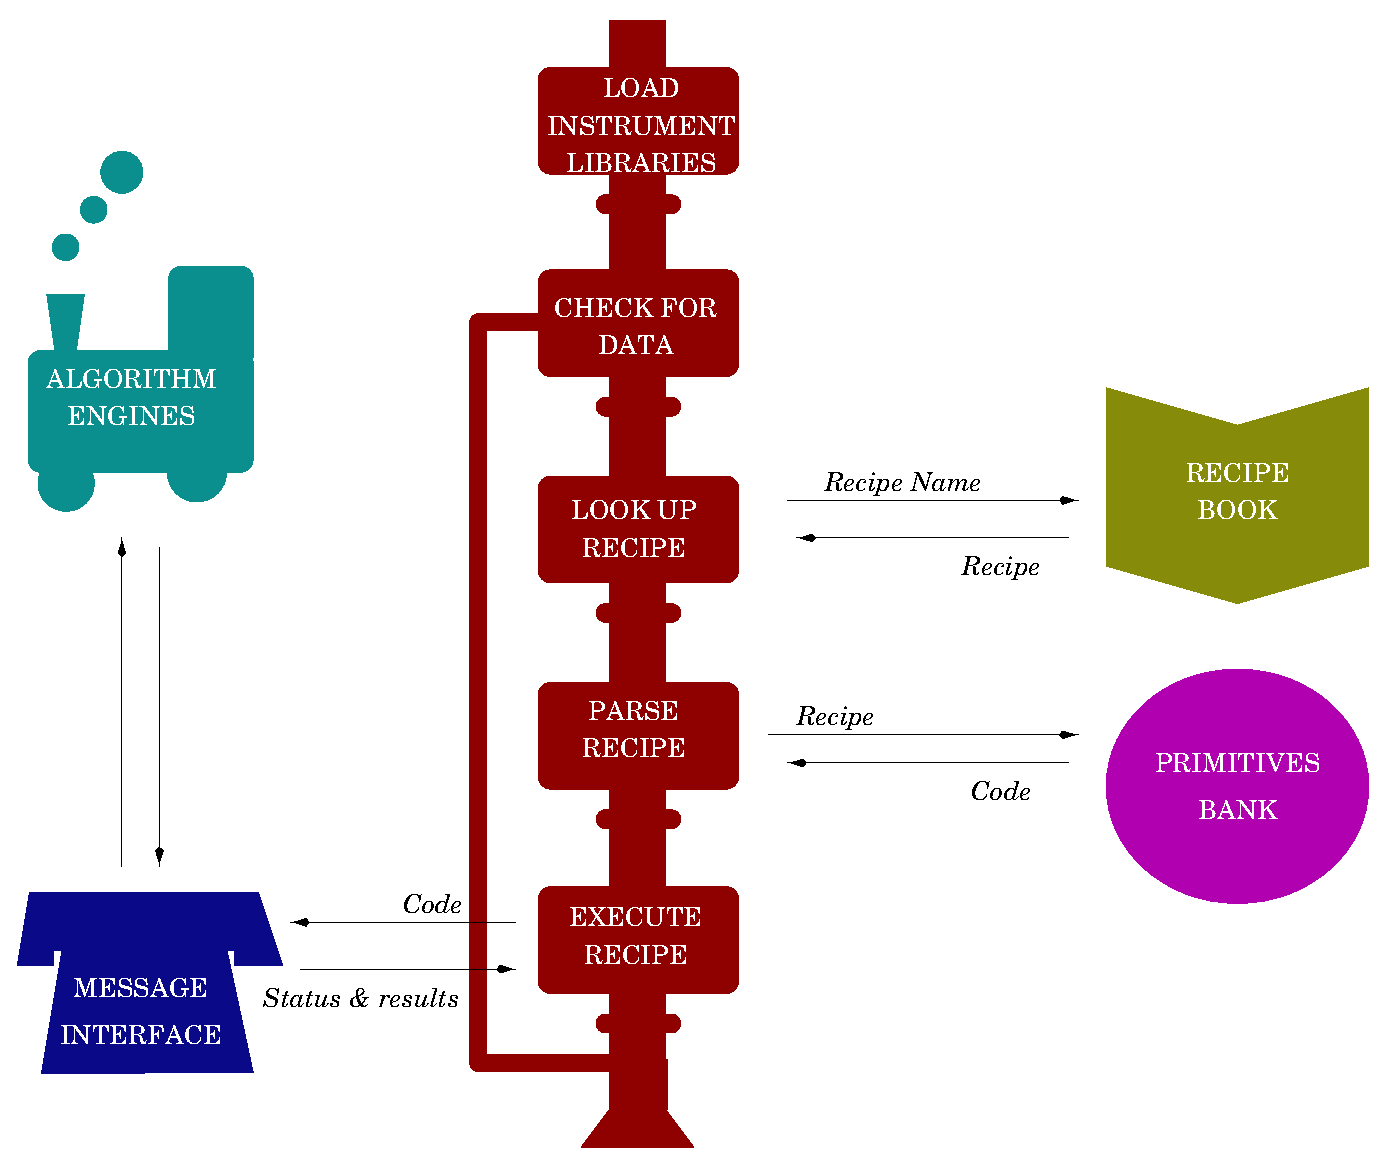
\includegraphics[width=\textwidth]{sun230_train.eps}
\caption{What happens in ORAC-DR}
\end{figure}


%% ORACDRDOC_HOWTO:SettingUp
\section{Setting up to run oracdr\label{Setting_up_to_run_oracdr}\index{Setting up to run oracdr}}


An ORAC-DR HOWTO

\subsubsection*{Description\label{Setting_up_to_run_oracdr_Description}\index{Setting up to run oracdr!Description}}


This document describes how to set up the ORAC-DR software for your
environment. ORAC-DR requires \texttt{tcsh} for full functionality from the
setup system. If \texttt{tcsh} is not available the startup scripts
(\texttt{oracdr\_ufti} etc) will not set the specified UT date (the argument
is ignored). In this case the \texttt{ORAC\_DATA\_IN} and \texttt{ORAC\_DATA\_OUT}
environment variables must be set up explicitly. Additionally, the
\texttt{oracdr} command must include the '\texttt{-ut}' option as specified in the
\texttt{oracdr} documentation.

\subsection*{The short way (Starlink and JAC users only)\label{Setting_up_to_run_oracdr_The_short_way_Starlink_and_JAC_users_only_}\index{Setting up to run oracdr!The short way (Starlink and JAC users only)}}
\begin{itemize}

\item

If your data conforms to the directory naming convention of the
instrument, type:

\begin{verbatim}
 setenv ORAC_DATA_ROOT <root data directory>
 oracdr_<instrument> YYYYMMDD
\end{verbatim}


You can set up this variable by hand or in your own login script
\textbf{before} running the oracdr instrument setup script.



For example, the naming convention for UFTI data is
\texttt{ufti\_data/YYYYMMDD/raw/} for the location of raw data and
\texttt{ufti\_data/YYYYMMDD/reduced/} for the location of reduced data. You can
set \texttt{ORAC\_DATA\_ROOT} to the directory in which the UT directory is
found. So if your raw UFTI data is in
\texttt{/home/user/data/UKIRT/ufti\_data/YYYYMMDD/raw/} you should type:

\begin{verbatim}
 setenv ORAC_DATA_ROOT /home/user/data/UKIRT/
 oracdr_ufti
 oracdr [-options] [RECIPE]
\end{verbatim}


in order to reduce your UFTI data.


\item

If your raw and reduced data are in arbitrary directories, type:

\begin{verbatim}
 oracdr_instrument <YYYYMMDD>
 setenv ORAC_DATA_IN <raw data directory>
 setenv ORAC_DATA_OUT <reduced data directory>
\end{verbatim}


e.g.

\begin{verbatim}
 oracdr_ufti 19990602
 setenv ORAC_DATA_IN /home/user/data/patt99/raw/
 setenv ORAC_DATA_OUT /scratch/user
 oracdr [-options] [RECIPE]
\end{verbatim}
\end{itemize}


Note that ORAC-DR works exclusively in \texttt{ORAC\_DATA\_OUT}, irrespective of
what your current directory is when you invoke it.

\subsection*{The long way\label{Setting_up_to_run_oracdr_The_long_way}\index{Setting up to run oracdr!The long way}}


ORAC-DR uses a number of environment variables for configuration. If
you are using a non-Starlink non-JAC installation of ORAC-DR, please
consult \emph{ShellVariables} (see appendix) for the complete set of
variables and their meaning.

\subsection*{Document info\label{Setting_up_to_run_oracdr_Document_info}\index{Setting up to run oracdr!Document info}}


Original author: frossie



\$Id\$


%% ORACDRDOC_HOWTO:Components
\section{ORAC-DR Components\label{ORAC-DR_Components}\index{ORAC-DR Components}}


An ORAC-DR HowTo

\subsection*{Description\label{ORAC-DR_Components_Description}\index{ORAC-DR Components!Description}}


This document describes the executables that form part of the ORAC-DR
distribution.

\subsection*{Set up scripts\label{ORAC-DR_Components_Set_up_scripts}\index{ORAC-DR Components!Set up scripts}}


These are the commands you have to type to set up ORAC-DR for the various
supported instruments.

\begin{description}

\item[{\texttt{oracdr\_cgs4}}] \mbox{}

Sets up for the data reduction of CGS4.


\item[{\texttt{oracdr\_ircam}}] \mbox{}

Sets up for the data reduction of IRCAM, the UKIRT Infrared Camera.


\item[{\texttt{oracdr\_michelle}}] \mbox{}

Sets up for the data reduction of MICHELLE.


\item[{\texttt{oracdr\_scuba}}] \mbox{}

Sets up for the data reduction of SCUBA, the JCMT Submillimetre Common
User Bolometer Array.


\item[{\texttt{oracdr\_ufti}}] \mbox{}

Sets up for the data reduction of UFTI (the UKIRT Fast Track Imager)


\item[{\texttt{oracdr\_iris2}}] \mbox{}

Sets up for the data reduction of IRIS-2 (the AAT Infrared Imaging
Spectrograph)


\item[{\texttt{oracdr\_uist}}] \mbox{}

Sets up the data-reduction system for UIST (The UKIRT infrared
imaging spectrometer with IFU).


\item[{\texttt{oracdr\_ingrid}}] \mbox{}

Sets up the data reduction system for INGRID.


\item[{\texttt{oracdr\_isaac}}] \mbox{}

Sets up the data-reduction system for ESO ISAAC in imaging modes.
Support for spectroscopy modes is ongoing.


\item[{\texttt{xoracdr}}] \mbox{}

Initialises the environment and then launches the ORAC-DR GUI.

\end{description}
\subsection*{Executables\label{ORAC-DR_Components_Executables}\index{ORAC-DR Components!Executables}}
\begin{description}

\item[{\texttt{oracdr}}] \mbox{}

Runs the pipeline. For more information see \emph{oracdr}


\item[{\texttt{oracman}}] \mbox{}

Displays man-page information for all ORAC-DR executables, recipes,
primitives and how-to guides. Type:

\begin{verbatim}
 oracman <foo>
\end{verbatim}


for documentation, e.g.

\begin{verbatim}
 oracman oracdr
 oracman ARRAY_TESTS
 oracman _SUBTRACT_DARK_
 oracman DisplaySystem
\end{verbatim}

\item[{\texttt{oracdisp}}] \mbox{}

Sets up the X display configuration tool. For more information on
\texttt{oracdisp} and the display system see \emph{oracdisp} and \emph{DisplaySystem}


\item[{\texttt{oracdr\_nuke}}] \mbox{}

Kills \texttt{oracdr}, any related processes (including any Starlink
processes), and clears shared memory owned by the user. Useful if
something happens to cause ORAC-DR to hang. See \textsf{oracdr\_nuke}

\end{description}
\subsection*{Document info\label{ORAC-DR_Components_Document_info}\index{ORAC-DR Components!Document info}}

%% ORACDRDOC_HOWTO:Xoracdr
\section{Xoracdr\label{Xoracdr}\index{Xoracdr}}


An ORAC-DR HOWTO

\subsection*{DESCRIPTION\label{Xoracdr_DESCRIPTION}\index{Xoracdr!DESCRIPTION}}


The ORAC-DR pipeline can be controlled from the Xoracdr
application. This note describes the user interface of Xoracdr and how
to use it.

\subsection*{STARTING XORACDR\label{Xoracdr_STARTING_XORACDR}\index{Xoracdr!STARTING XORACDR}}


The ORAC-DR pipeline and Xoracdr software uses a number of
environmental variables for configuration. For non-Starlink, non-JAC
installation of ORAC-DR, please consult \emph{ShellVariables} (see
appendix) for more information.



To start the Xoracdr application type \texttt{xoracdr} at the prompt:

\begin{verbatim}
  % xoracdr
  ORAC Data Reduction Pipeline -- (ORAC-DR Version 3.0)
\end{verbatim}
\begin{verbatim}
  Please wait, spawning Xoracdr...
\end{verbatim}


this will run the Xoracdr setup script and bring up the Xoracdr main window.

\subsection*{OPTIONS AND ARGUMENTS\label{Xoracdr_OPTIONS_AND_ARGUMENTS}\index{Xoracdr!OPTIONS AND ARGUMENTS}}


Unlike command line control of the ORAC-DR pipeline, configuration of
the pipeline options is via the main window. There are therefore only
a few command line options

\begin{description}

\item[{\textbf{-vers}}] \mbox{}

Displays revision information about Xoracdr and the version of Perl it
is using.


\item[{\textbf{-ut} \textit{YYYYMMDD}}] \mbox{}

UT date of observations (defaults to current YYYYMMDD).The UT is
required for UKIRT and JCMT instruments as it forms part of the file
naming convention for data files.


\item[{\textbf{-honour}}] \mbox{}

If you start xoracdr with the \texttt{ORAC\_INSTRUMENT} environment variable
unset, i.e. you have not run one of the instrument setup scripts, but
have the \texttt{ORAC\_DATA\_OUT} environment variable set you may wish to
force Xoracdr to honour this using the \texttt{-honour} command line option.

\end{description}
\subsection*{USING XORACDR\label{Xoracdr_USING_XORACDR}\index{Xoracdr!USING XORACDR}}


If your data conforms to the directory naming convention for the
instrument, setting up the pipeline is fairly trivial.



Select your instrument from the list box to the left hand side of the
application main window and then enter the UT date of the observations
you are reducing into the entry field in the center of the main
window. The raw and reduced data paths should now be set
correctly. Enter the range of frame numbers that you are interested in
into the \texttt{List} text entry and push the \texttt{Start ORAC-DR} button. The
pipeline should initalise and start processing you data immediately.



A more detailed description of the Xoracdr user interface follows for
those people who need to do something slightly out of the ordinary,
although the interface itself should be fairly self explanatory for
those people used to the \emph{oracdr} command line interface.

\subsection*{THE MAIN WINDOW\label{Xoracdr_THE_MAIN_WINDOW}\index{Xoracdr!THE MAIN WINDOW}}


The Xoracdr main window is divided into three main sections. At the
top is the menu bar with \texttt{File}, \texttt{Display}, \texttt{Options}, \texttt{Recipe}
and \texttt{Help} menus.

\begin{figure}
\begin{center}
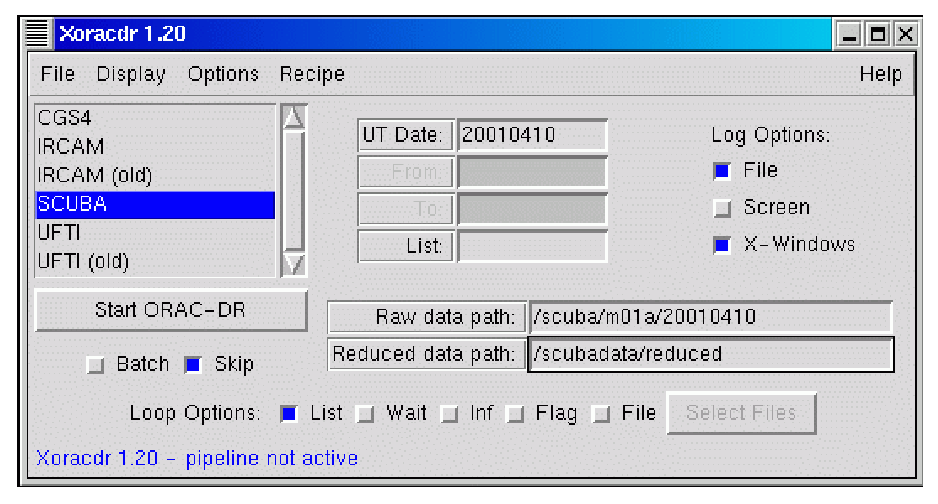
\includegraphics[width=5.0in]{sun230_xoracdr.eps}
\caption{The Xoracdr main window}
\end{center}
\end{figure}

\begin{description}

\item[{File Menu}] \mbox{}\begin{description}

\item[{Stop Processing}] \mbox{}

When the pipeline is running further data processing can be halted by
selecting this menu entry. Control will be returned to the main
window, processing can be restarted from the beginning by depressing
the \textit{Start ORAC-DR} button.


\item[{Pause Processing}] \mbox{}

When the pipeline is running the processing of further data can be
paused by selecting this menu item, a pop-up window will appear with a
\textit{Resume} button. Processing can be re-started by depressing the
\textit{Resume} button in the pop-up.


\item[{Nuke ORAC-DR}] \mbox{}

Selecting this menu option will kill all ORAC-DR related processes,
including spawned Starlink monoliths, and will free up any shared
memory used by these processes. This will also kill the Xoracdr
graphical user interface.

\end{description}

\item[{Display Menu}] \mbox{}\begin{description}

\item[{No Display}] \mbox{}

Selecting this checkbox will instruct Xoracdr not to launch the
display system. No data will be displayed and GWM (or GAIA) windows
will not be launched.


\item[{Configure Display}] \mbox{}

Allows configuration of the ORAC-DR display environment. Selecting
this menu item will display a popup window which can be used to edit
the current environment and add display directives to the current
environment. This popup can also be run as a stand alone application
from the command line, e.g.

\begin{verbatim}
  % oracdisp
\end{verbatim}


for more information on how to use the display environment editor see
the \emph{oracdisp} documentation and the documentation on the
\emph{DisplaySystem}.

\end{description}

\item[{Options Menu}] \mbox{}\begin{description}

\item[{Allow Resume}] \mbox{}

Allow the pipeline to resume midway through the processing of a group
so long as the recipe/instrument supports this behaviour. Default is
for the group file to be deleted when a new group is created. When
this menu option is selected, the group file is retained. \textbf{NOTE} this
option is not currently supported by IRCAM, UFTI and SCUBA recipes.


\item[{No Engines}] \mbox{}

Do not start algorithm engines. \textbf{NOTE} this will cause the vast
majority of recipes to fail.


\item[{Common ADAM}] \mbox{}

Do not create an invocation specific temporary directory for the
messaging systems but use whatever directory is the usual default. For
ADAM tasks this would mean that \texttt{\~{}}/adam or \texttt{\$ADAM\_USER} will be used
rather than a private ORAC-DR directory. This should only be used when
it is required for ORAC-DR to talk to tasks that were not started by
the pipeline and could lead to possible confusion if multiple
pipelines are running using this flag.


\item[{Verbose}] \mbox{}

If selected then messages from the Starlink engines will be printed in
addition to the normal ORAC-DR messages


\item[{Debug}] \mbox{}

Log debug messages to file \texttt{ORACDR.DEBUG} in \texttt{\$ORAC\_DATA\_OUT}.


\item[{Warn}] \mbox{}

Turn on perl level warning messages (\texttt{perl -w}). This should be used
for debugging only. If \texttt{-verbose} is also true then full perl
diagnostics are turned on (see \emph{diagnostics} for more information on
this perl pragma).


\item[{Beep}] \mbox{}

Is selected the pipeline will make as much noise as possible over
errors and pipeline exit.


\item[{Setup Environment}] \mbox{}

If selected a window will appear allowing you to enter file paths for
the data and calibration root directories, user recipe and primitive
directories, the raw and reduced data directories and the instrument
calibration directory. If these have already been set, either by
selecting an instrument from the listbox or from environment variables
you can override the default options using this popup window. \textbf{NOTE}
The raw and reduced data paths will be overridden if you select an
instrument from the main window listbox after entering values into
this window.


\item[{Calibration Options}] \mbox{}

This item will remain disabled until an instrument is selected in the
main window listbox, after this you are free to select this item from
the menu. On selection a window will popup allowing you to enter
calibration options for the instrument, see the user guide for your
instrument for more information.

\end{description}

\item[{Recipe Menu}] \mbox{}\begin{description}

\item[{Show Current Recipe}] \mbox{}

Selecting this menu item will ensure that the recipe display window
will appear along with the log window. The recipe display window will
show the currently executing recipe and a list of the primitives
contained in the recipe. The currently running primitive will be
highlighted.


\item[{Override: \textit{RECIPE}}] \mbox{}

This item will be greyed out until an override recipe is selected
using the \textit{Override Recipe} option further down the \texttt{Recipe}
menu. After an override recipe is selected then this option will
become active. If the checkbox is selected then the selected recipe
will override the one specified in the file headers. This override
recipe is used for all data files regardless of header contents or
observation mode, so make sure you only only apply it to appropriate
data frames.


\item[{Set Override Recipe}] \mbox{}

This item will remain disabled until an instrument is selected in the
main window listbox, after which if selected it will allow you to
choose an \textit{Override Recipe}


\item[{Edit Recipe}] \mbox{}

Allows you to select and then edit a recipe. The recipe will be saved
to \texttt{ORAC\_RECIPE\_DIR}, the user recipe directory, which if unset will
default to \texttt{ORAC\_DATA\_OUT}. Recipes in \texttt{ORAC\_RECIPE\_DIR} will be run
in preference to those in the instrument recipe directories of the
same name.

\end{description}

\item[{Help Menu}] \mbox{}

Selecting an entry from the \texttt{Help} menu will popup a help browser to
display the relevant documentation. At the bottom on the menu there is
also an \texttt{About XORAC-DR} entry which will display the licence terms
and conditions for the ORAC-DR software.

\end{description}


At the bottom of the main window is the status bar, this reports the
status of the pipeline process. It will display the currently running
recipe name, along with other status information.



Between the menu and status bar is the bulk of the main window. On the
left is the instrument list box, this allows you to select the
instrument whose data you wish to process. If the \texttt{ORAC\_INSTRUMENT}
environment variable is set before starting Xoracdr the instrument
will be preselected on startup.



Once an instrument is selected the user interface will be configured
into a default state for the instrument. \textbf{NOTE} it is important to
select an instrument before doing any customization of the settings as
your changes may be overridden by the default options imposed by
setting up an instrument.



At this point the \textit{Start ORAC-DR} button will become enabled and you
can start the pipeline if the configuration options are to your
liking.

\subsection*{FURTHER CONFIGURATION\label{Xoracdr_FURTHER_CONFIGURATION}\index{Xoracdr!FURTHER CONFIGURATION}}


If not already set using the \texttt{-ut} command line option, and if you
are using a loop type where it is necessary to build the filename
using the UT date (i.e. all loop options except \textit{file}) the UT date
of the observation run can be set via the relevant text entry box in
the middle of the main window. \textbf{NOTE} Doing so will run the
instrument setup routine again which will override some environment
options such as \texttt{ORAC\_DATA\_IN} and \texttt{ORAC\_DATA\_OUT}.



If ORAC-DR is being run in post-observation mode, the default data
detection loop is \textit{list}. Other loop options can be selected using
the series of checkboxes along the bottom of the main window. The
available options are

\begin{description}

\item[{\textbf{list}}] \mbox{}

The pipeline will stop once the observations in the list have been
reduced.


\item[{\textbf{wait}}] \mbox{}

Waits for data to appear before timing out. Data is reduced and the
pipeline waits for the next file.


\item[{\textbf{inf}}] \mbox{}

Do not wait for data. Simply reduce data starting with observation
specified by \texttt{from} and continuing until no more files are present.
This is the fastest way of reducing data offline.


\item[{\textbf{flag}}] \mbox{}

Waits for completion files to appear (flags) before processing the
data.  Data is reduced and the pipeline waits for more data by
checking the presence of a flag.


\item[{\textbf{file}}] \mbox{}

Works much like the \texttt{list} loop option except that looping is carried
out over a list of arbitrarily named files. When the \texttt{file} loop option
is selected the \textit{Select Files} button will be enabled allowing you to
generate this list. \textbf{NOTE} As well as having arbitrary filenames,
files can be added in arbitrary order, this allows you to reduces (for
instance) all the calibration frames for a night first, followed by
the actual observations.

\end{description}


There are, in addition, two other options which affect the looping
scheme, these being \texttt{batch} and \texttt{skip}.

\begin{description}

\item[{\textbf{batch}}] \mbox{}

Run in batch mode. Precalculate groups before processing data. `wait'
loop mode should not be used with this option.  \textbf{NOTE} only SCUBA
recipes support this option.


\item[{\textbf{skip}}] \mbox{}

Allow the data detection loop to skip missing observations. Default is
to stop the loop when an expected file can not be found.

\end{description}


See the \emph{DataLoops} documentation for more information on looping
schemes.

\subsection*{LOG OPTIONS\label{Xoracdr_LOG_OPTIONS}\index{Xoracdr!LOG OPTIONS}}


Finally, you can configure the log options from the three checkboxes
located to the right hand side of the main window. By default logging
is sent to a file and to an Xwindow.

\subsection*{SEE ALSO\label{Xoracdr_SEE_ALSO}\index{Xoracdr!SEE ALSO}}


\emph{oracdr}, \emph{oracdisp}, \textsf{oracdr\_parse\_recipe}

\subsection*{AUTHOR\label{Xoracdr_AUTHOR}\index{Xoracdr!AUTHOR}}


Alasdair Allan (aa@astro.ex.ac.uk)

\subsection*{COPYRIGHT\label{Xoracdr_COPYRIGHT}\index{Xoracdr!COPYRIGHT}}


Copyright (C) 1998-2001 Particle Physics and Astronomy Research Council.
All Rights Reserved.

\subsection*{REVISION\label{Xoracdr_REVISION}\index{Xoracdr!REVISION}}
\begin{verbatim}
 $Id$
\end{verbatim}

%% ORACDRDOC_BIN:oracdr
\section{oracdr\label{oracdr}\index{oracdr}}


ORAC Data Reduction pipeline

\subsection*{Synopsis\label{oracdr_Synopsis}\index{oracdr!Synopsis}}
\begin{verbatim}
  oracdr [-options] [RECIPE]
  oracdr -from 5
  oracdr -ut 19990523 -list 15:35,40,44 -batch
\end{verbatim}
\subsection*{DESCRIPTION\label{oracdr_DESCRIPTION}\index{oracdr!DESCRIPTION}}


\texttt{oracdr} is the actual ORAC-DR data reduction pipeline.
This document describes the command line options that
can be used to modify the pipeline operation.

\subsection*{Arguments\label{oracdr_Arguments}\index{oracdr!Arguments}}


The following argument  is  supported:

\begin{itemize}

\item RECIPE

By default, ORAC-DR looks in the file header for the name of the
recipe to be used on the data. If you specify the name of a recipe on
the command line, it will override the one specified in the
header. This override recipe is used for all data files regardless of
header contents or observation mode, so make sure you only only apply
it to appropriate data frames.

\end{itemize}
\subsection*{Options\label{oracdr_Options}\index{oracdr!Options}}


All ORAC-DR behaviour is controlled by the option
switches. These options may be abbreviated to a unique substring. It
is via command line switches that you (for example) control the range
of file numbers to be reduced, force the system to use a particular
calibration file when reducing (e.g. to try a different flat
exposure). This list needs to be read thoroughly by anyone wanting to
use the system.

\subsubsection*{General Options\label{oracdr_General_Options}\index{oracdr!General Options}}
\begin{description}

\item[{\textbf{-help}}] \mbox{}

List help text. This prints a summary of this document.


\item[{\textbf{-version}}] \mbox{}

Print the version number.


\item[{\textbf{-verbose}}] \mbox{}

Print messages from the Starlink engines (rather than just ORAC-DR
messages).


\item[{\textbf{-man}}] \mbox{}

Print the full documentation.


\item[{\textbf{-debug}}] \mbox{}

Log debug messages to file \texttt{ORACDR.DEBUG} in \texttt{\$ORAC\_DATA\_OUT}.


\item[{\textbf{-warn}}] \mbox{}

Turn on perl level warning messages (\texttt{perl -w}). This should be
used for debugging only. If \texttt{-verbose} is also true then full
perl diagnostics are turned on (see \emph{diagnostics} for more information
on this perl pragma).


\item[{\textbf{-beep}}] \mbox{}

Make as much noise as possible over errors and pipeline exit.
Default is not to beep.

\end{description}
\subsubsection*{Windows and output\label{oracdr_Windows_and_output}\index{oracdr!Windows and output}}
\begin{description}

\item[{\textbf{-nodisplay}}] \mbox{}

Do not launch the display system. No data will be displayed and GWM,
GAIA etc. windows will not be launched.


\item[{\textbf{-showcurrent}}] \mbox{}

Launch a recipe viewer window along with the log Xwindow


\item[{\textbf{-log s}}] \mbox{}

Log to terminal screen (standard out)


\item[{\textbf{-log f}}] \mbox{}

Log to a file. The logfile is called \texttt{.oracdr\_NNNN.log} where NNNN
is the current process ID. It is written to \texttt{\$ORAC\_DATA\_OUT} and is
a hidden file.


\item[{\textbf{-log x}}] \mbox{}

Log to an Xwindow. Has the advantage that warnings and errors are
written to different, independently scrollable windows.

\end{description}


The three log options can be combined. The default is \texttt{-log sx}



To run ORAC-DR using output only within the xterm that you used
to invoke it in, use \texttt{-nodisplay -log s}. This is the fastest way
to run the pipeline if you are not interested in visually
inspecting the data as it is being reduced.

\subsubsection*{Observations\label{oracdr_Observations}\index{oracdr!Observations}}
\begin{description}

\item[{\textbf{-from}}] \mbox{}

Number of first observation.


\item[{\textbf{-to}}] \mbox{}

Number of last observation.


\item[{\textbf{-list}}] \mbox{}

Comma separated list of observation \textit{numbers}. Colons indicate a range.
For example, `1,2,4:6,10' means 1,2,4,5,6,10.


\item[{\textbf{-files}}] \mbox{}

File name (relative to current directory) of a flat ASCII text file containing
a list of observation \textit{files} to be reduced, one file per line.

\end{description}
\subsubsection*{UT date\label{oracdr_UT_date}\index{oracdr!UT date}}
\begin{description}

\item[{\textbf{-ut}}] \mbox{}

UT date of observations (defaults to current yyyymmdd). When the
instrument specific setup scripts are run, oracdr is automatically
aliased to use the correct \texttt{-ut} option. The UT is required for
UKIRT and JCMT instruments as it forms part of the file naming
convention for data files.

\end{description}
\subsubsection*{Recipe Selection and Modification\label{oracdr_Recipe_Selection_and_Modification}\index{oracdr!Recipe Selection and Modification}}
\begin{description}

\item[{\textbf{-recsuffix}}] \mbox{}

Modify the recipe search algorithm such that a recipe variant can be
selected if available. For example with `\texttt{-recsuffix QL}' a recipe
named MYRECIPE\_QL would be picked up in preference to MYRECIPE.



Multiple suffices can be supplied using a comma separator.

\begin{verbatim}
 -recsuffix QL1,QL2
\end{verbatim}

\item[{\textbf{-recpars}}] \mbox{}

Recipe behaviour can be controlled by specifying a recipe parameters
file. This is a file in INI format with a block per recipe name.

\begin{verbatim}
 [RECIPE_NAME]
 param1=value1
 param2=value2
\end{verbatim}
\end{description}
\subsubsection*{Calibration options.\label{oracdr_Calibration_options_}\index{oracdr!Calibration options.}}
\begin{description}

\item[{\textbf{-calib}}] \mbox{}

Used to specify calibration overrides. Accepts comma separated key=value
pairs. (e.g. `\texttt{-cal dark=file1}' or `\texttt{-cal dark=file1,bias=file2}'). The
allowed options depends on the instrument that is in use.

\end{description}


See \emph{Calibrating} for more information on how the pipeline deals
with calibrations.

\subsubsection*{Looping options\label{oracdr_Looping_options}\index{oracdr!Looping options}}


The \texttt{-loop} option specifies the type of data detection loop. Allowed
values are `list', `inf', `wait', `flag' or 'file'. In almost all cases of
offline use, `inf' is most appropriate.

\begin{description}

\item[{\textbf{-loop list}}] \mbox{}

Default when using the \texttt{-list} option. The pipeline will stop
once the observations in the list have been reduced.


\item[{\textbf{-loop wait}}] \mbox{}

Waits for data to appear before timing out. Data is reduced and the pipeline
waits for the next file.


\item[{\textbf{-loop inf}}] \mbox{}

Do not wait for data. Simply reduce data starting with observation
specified by \texttt{-from} and continuing until no more files are present.
Implicitly used when \texttt{-from} is specified. This is the fastest way
of reducing data offline.


\item[{\textbf{-loop flag}}] \mbox{}

Waits for completion files to appear (flags) before processing the data.
Data is reduced and the pipeline waits for more data by checking the
presence of a flag.


\item[{\textbf{-loop file}}] \mbox{}

Works much like \texttt{-loop list} except that looping is carried out over a
list of arbitarly named files input from the \texttt{-files} command line option.


\item[{\textbf{-loop task}}] \mbox{}

Obtain data from a remote (DRAMA) task.

\end{description}


See \emph{DataLoops} for more
information on looping schemes.

\subsubsection*{Group processing options\label{oracdr_Group_processing_options}\index{oracdr!Group processing options}}
\begin{description}

\item[{\textbf{-batch}}] \mbox{}

Run in batch mode. Precalculate groups before processing
data. `wait' loop mode should not be used with this option.
\textbf{NOTE} only SCUBA recipes support this option.


\item[{\textbf{-skip}}] \mbox{}

Allow the data detection loop to skip missing observations.
Default is to stop the loop when an expected file can not be found.


\item[{\textbf{-resume}}] \mbox{}

Allow the pipeline to resume midway through the processing
of a group. (so long as the recipe/instrument supports
this behaviour). Default is for the group file to be deleted
when a new group is created. When \texttt{-resume} is set, the group
file is retained. \textbf{NOTE} this option is not currently supported by
IRCAM, UFTI and SCUBA recipes.


\item[{\textbf{-grptrans}}] \mbox{}

Groups are presumed to be transinet and no longer needed when a new
group is created.  This is useful when you know that groups can not be
broken up. Has no effect in batch mode. Memory usage will be
significantly lower if many hundreds of frames and groups are to be
processed.



This option is not the same as setting the ORAC\_NOGROUPS environment
variable. That environment variable disables all group processing
whereas this command line option ensures that only a single group
is being processed.


\item[{\textbf{-onegroup}}] \mbox{}

All given observations and files are processed in the same group. Be
careful in using this option, as sometimes this may not be what you
want (i.e. if you're processing ACSIS data at two different
frequencies).

\end{description}
\subsubsection*{Engine Options\label{oracdr_Engine_Options}\index{oracdr!Engine Options}}
\begin{description}

\item[{\textbf{-noeng}}] \mbox{}

Do not start algorithm engines. \textbf{NOTE} this will cause
the vast majority of recipes to fail.


\item[{\textbf{-nomsgtmp}}] \mbox{}

Do not create an invocation specific temporary directory for the
messaging systems but use whatever directory is the usual default. For
ADAM tasks this would mean that \texttt{\~{}}/adam or \$ADAM\_USER will be used
rather than a private ORAC-DR directory. This should only be used when
it is required for ORAC-DR to talk to tasks that were not started by
the pipeline and could lead to possible confusion if multiple
pipelines are running using this flag.

\end{description}
\subsection*{REVISION\label{oracdr_REVISION}\index{oracdr!REVISION}}


\$Id\$

\subsection*{AUTHORS\label{oracdr_AUTHORS}\index{oracdr!AUTHORS}}


Frossie Economou (frossie@jach.hawaii.edu),
Tim Jenness (t.jenness@jach.hawaii.edu),
Alasdair Allan (aa@astro.ex.ac.uk),
Brad Cavanagh (b.cavanagh@jach.hawaii.edu)

\subsection*{COPYRIGHT\label{oracdr_COPYRIGHT}\index{oracdr!COPYRIGHT}}


Copyright (C) 1998-2008 Science and Technology Facilities Council.
All Rights Reserved.



This program is free software; you can redistribute it and/or modify it under
the terms of the GNU General Public License as published by the Free Software
Foundation; either version 3 of the License, or (at your option) any later
version.



This program is distributed in the hope that it will be useful,but WITHOUT ANY
WARRANTY; without even the implied warranty of MERCHANTABILITY or FITNESS FOR A
PARTICULAR PURPOSE. See the GNU General Public License for more details.



You should have received a copy of the GNU General Public License along with
this program; if not, write to the Free Software Foundation, Inc., 59 Temple
Place,Suite 330, Boston, MA  02111-1307, USA


%% ORACDRDOC_HOWTO:Credits
\section{ORAC-DR\label{ORAC-DR}\index{ORAC-DR}}


Credit and License

\subsection*{Description\label{ORAC-DR_Description}\index{ORAC-DR!Description}}


This document describes the credit and licensing information for ORAC-DR.

\subsection*{Acknowledgements\label{ORAC-DR_Acknowledgements}\index{ORAC-DR!Acknowledgements}}


ORAC-DR was developed at the Joint Astronomy Centre by
Frossie Economou and Tim Jenness in collaboration with the
UK Astronomy Technology Centre as part of the ORAC project.
Other members of the ORAC-DR team have subsequently contributed
to ORAC-DR's infrastructure.



Other members of the ORAC team provided invaluable scientific
and technical input to ORAC-DR, in particular Alan Bridger (UKATC),
Gillian Wright (UKATC) and Andy Adamson (JAC).



Software support for SCUBA was added by Tim Jenness.  Malcolm Currie
provided the software for UFTI, IRCAM, and Michelle imaging.  Support
for CGS4 and Michelle spectroscopy was added by Paul Hirst, Frossie
Economou, Tim Jenness, Malcolm Currie, and Brad Cavanagh.  The ORAC-DR
GUI was added by Alasdair Allan (Starlink). IRIS-2 support was added
by Brad Cavanagh in conjunction with Stuart Ryder (AAT). ISAAC and
INGRID support was added by Malcolm Currie. UIST IFU support was added
by Stephen Todd.



The developers are also grateful to numerous members of UKIRT and JCMT
staff for their ideas and feedback.

\subsection*{Copyright and License\label{ORAC-DR_Copyright_and_License}\index{ORAC-DR!Copyright and License}}


ORAC-DR is copyright (C) 1998-2003 PPARC (the UK Particle Physics and Astronomy
Research Council). It is distributed by Starlink under the
GNU General Public License as published by the Free Software Foundation.



If you have used ORAC-DR for your data reduction please acknowledge it
in your publications.  It costs you nothing and gives us a warm fuzzy
feeling.

\subsection*{Document info\label{ORAC-DR_Document_info}\index{ORAC-DR!Document info}}

\section{Release Notes}

\begin{description}

\item[V4.0]

\begin{itemize}

\item Support for UIST in all observation modes.

\item Support for INGRID in all observation modes.

\item Support for ISAAC in imaging mode, and preliminary support for
spectroscopy mode.

\item New document, \xref{SUN/246}{sun246}{}, describing integral field
  spectroscopy reduction and recipes.

\item New \texttt{ORAC\_KEEP} environment variable to retain intermediate
  frames.

\item Spectroscopy:

\begin{itemize}

\item Widened optimal extraction windows for better profile fitting.

\item Flux calibration for I-band.

\end{itemize}

\item Imaging:

\begin{itemize}

\item Modification of EXTRACTOR object-detection parameters to obtain a
    flatter, more accurate flat-fielded mosaic.

\item Offset patterns need not be centered at centre of the array.

\item Four new recipes including NOD\_SKY\_FLAT\_THERMAL recipe for reduction
    of thermal data using sky observations for flat-fielding.

\item REDUCE\_DARK supports variance creation and propagation by default.

\item Expanded \xref{SUN/232}{sun232}{} with more description of the
  primitives, and information for programmers wishing to adapt the recipes.

\end{itemize}

\item SCUBA:

\begin{itemize}

\item CSO Tau fits up-to-date to January 2003 (when the tau meter broke).

\item Flux Conversion Factors verified up to March 2003.

\item More robust error handling for poor data.

\end{itemize}

\end{itemize}

\item[V3.1]

\begin{itemize}

\item Support for AAT IRIS2 data

\item Spectroscopy:

\begin{itemize}

\item Extracts "sky-arcs" to enable wavelength calibration of Michelle data.

\item Now handles offset patterns that don't originate at (0,0).

\item Peak-up routines for Michelle.

\item Single beam polarimetry now much more robust.

\item Masking of off-slit areas of image improved.

\item Better bad pixel detection in flat fields.

\end{itemize}

\item Imaging:

\begin{itemize}

\item Addition of NOD\_CHOP\_FAINT (faint mid-IR) and
    NOD\_CHOP\_SCAN (scan pattern mid-IR) recipes.

\item Addition of ADDWCS (adds WCS to headers) recipe.

\end{itemize}

\end{itemize}

\item[V3.0]

\begin{itemize}

\item Support for Michelle data.

\item Support for multi-mode instruments, such as Michelle and UIST.

\item Three Michelle recipes for nodded and chopped data (vanilla,
  photometry and moving target).  New NQ standards file.

\item Easy to switch on variance creation and propagation; calculates
  correct data variance for UKIRT IR imagers.

\item  Faster object masking using EXTRACTOR instead of PISA.

\item Better registration of sparse fields using astrometry.

\item Tidier output for easier reading.  Added content to messages.

\item Comments in calibration rules files.

\item SCUBA: improvements in calibration of SCUBA data (both for flux
    conversion factors and extinction correction using
     \texttt{--calib tausys=csofit}).

\item Use of internal headers and directory reorganisation, permitting
     generic-named recipes and primitives, and optimising code use;
     and easier to add new instruments.

\end{itemize}

\item[V2.1]

\begin{itemize}

\item New GUI (xoracdr) to simplify use of the pipeline.

\item Enhanced CGS4 and imaging recipes.

\end{itemize}

\item[V2.0]

\begin{itemize}

\item Support for CGS4

\item SCUBA: Jiggle map calibration

\item IR Imaging: Polarimetry support plus recipe generalization.

\end{itemize}

\item[V1.0]

\begin{itemize}

\item First release to Starlink. Includes SCUBA and imaging (UFTI FITS
and IRCAM) recipes.

\end{itemize}

\end{description}


\appendix


%% ORACDRDOC_HOWTO:DataLoops
\section{The ORAC-DR Data Loops\label{The_ORAC-DR_Data_Loops}\index{The ORAC-DR Data Loops}}


An ORAC-DR HOWTO

\subsubsection*{Description\label{The_ORAC-DR_Data_Loops_Description}\index{The ORAC-DR Data Loops!Description}}


ORAC-DR may use a variety of ways to detect available data. This
document describes what they mean and when to use them.

\subsubsection*{How the pipeline operates\label{The_ORAC-DR_Data_Loops_How_the_pipeline_operates}\index{The ORAC-DR Data Loops!How the pipeline operates}}


ORAC-DR is a data-driven pipeline. This means that it does things in
response to incoming data and uses the information associated with
that data to determine how to process a file. It is also a sequential
(i.e. non-parallel) process. This means it only does one thing at a
time. As a result, ORAC-DR is always doing one of two things

\begin{itemize}

\item

Seeks new data


\item

Reduces data

\end{itemize}
\subsubsection*{How the pipeline detects new data\label{The_ORAC-DR_Data_Loops_How_the_pipeline_detects_new_data}\index{The ORAC-DR Data Loops!How the pipeline detects new data}}


Unless the \texttt{-file} option is used, the pipeline starts from looking for observation number 1, unless another number has been specified via the
\texttt{-from} or \texttt{-list} options.



The various \texttt{-loop} options determine what the criterion is for
concluding that the observation it is waiting for has indeed arrived.

\begin{description}

\item[{-loop wait}] \mbox{}

If you use this option, the pipeline monitors the size of the file
that is is expecting. For example, if it has just reduced observation
number 41, it waits for observation number 42 to appear on disk and
watches it size growing as it is being written out by the data
handling system. If the file does not grow in size for a certain
amount of time it concluded that readout is complete and proceeds with
reducing it. Obviously this method is not very robust if the pipeline
is operating or network-mounted disks or with acquisition systems that
are prone to stalling during readout. However it may be the only
option for online data reduction with some data handling systems. This
option should be used with IRCAM.


\item[{-loop flag}] \mbox{}

This option instructs the pipeline to monitor not the data file
itself, but a ``flag'' file whose appearance indicates readout
completion. Typically this is a zero-length file written by the data
acquisition after the data file writing is done. This is most robust
in architectures where there is no chance of a data file being written
without a flag file or vice versa. This option should be used with SCUBA,
UFTI, the WFS and MICHELLE.


\item[{-loop inf}] \mbox{}

Under this option, the pipeline reduces data assuming it is available
and keeps going one observation at a time until no more data is to be
found (or infinity, whichever comes first!), at which point it
terminates. It overrides the \texttt{-to} option. This is suitable for offline
data reduction of any instrument and is the default option if none is
specified.


\item[{-loop list}] \mbox{}

The specified data frames (and/or range of observations) are assumed
to be available, are reduced and then the pipeline exits. This option
is implied by usage of the \texttt{-list} option, or usage of the \texttt{-from}
and \texttt{-to} options in the same invocation. It is unlikely that a user
will need to explicitly specify it.


\item[{-loop file}] \mbox{}

The specified data frames are assumed available, are reduced and then
the pipeline exists. This option is impled by usage of the \texttt{-file}
option. Which provides a filename (relative to the current directory) of
a flat ASCII text file containing a list of observation \textit{files} to be
reduced, one filename per line. The filenames, unlike other loop options
used by ORAC-DR, are not based on UT date and may be arbitarily constructed.

\end{description}

%% ORACDRDOC_HOWTO:DisplaySystem
\section{The ORAC-DR Display System\label{The_ORAC-DR_Display_System}\index{The ORAC-DR Display System}}


An ORAC-DR HOWTO

\subsubsection*{Description\label{The_ORAC-DR_Display_System_Description}\index{The ORAC-DR Display System!Description}}


The ORAC-DR pipeline has a highly configurable display engine. This
note describes how it works and how to use it.

\subsubsection*{The \emph{disp.dat} file\label{The_ORAC-DR_Display_System_The_disp_dat_file}\index{The ORAC-DR Display System!The disp.dat file}}


The actual display engine is configured via an ASCII file called
\emph{disp.dat}. A default \emph{disp.dat} file exists in the general oracdr
distribution (\texttt{ORAC\_DIR}). Additionally a default \emph{disp.dat} is provided
by your instrument scientist or software engineer in the appropriate
calibration directory (\texttt{ORAC\_DATA\_CAL})



When you invoke oracdr, the pipeline checks in \texttt{ORAC\_DATA\_OUT} for an
existing \emph{disp.dat}. If it does not find one, it copies in the one from
\texttt{ORAC\_DATA\_CAL}, or if that doesn't exist, the one from \texttt{ORAC\_DIR}. In
all of those scenarios you end up with a file in \texttt{ORAC\_DATA\_OUT} which
is what is used by the display system. Any configuration changes have
to be reflected in the file.

\subsubsection*{How to change the \emph{disp.dat} file\label{The_ORAC-DR_Display_System_How_to_change_the_disp_dat_file}\index{The ORAC-DR Display System!How to change the disp.dat file}}


As it is an ASCII file, you may edit the file directly in your
favourite editor. However a much easier approach is to type use the
oracdisp GUI (simply type oracdisp). This has various options
available at the top and shows the \emph{disp.dat} entries corresponding to
those choices at the bottom. Don't forget to write press the
``Configure'' button to write the file to disk.



You may use oracdisp (or the editor) to change the display parameters
while the pipeline is running.

\begin{figure}
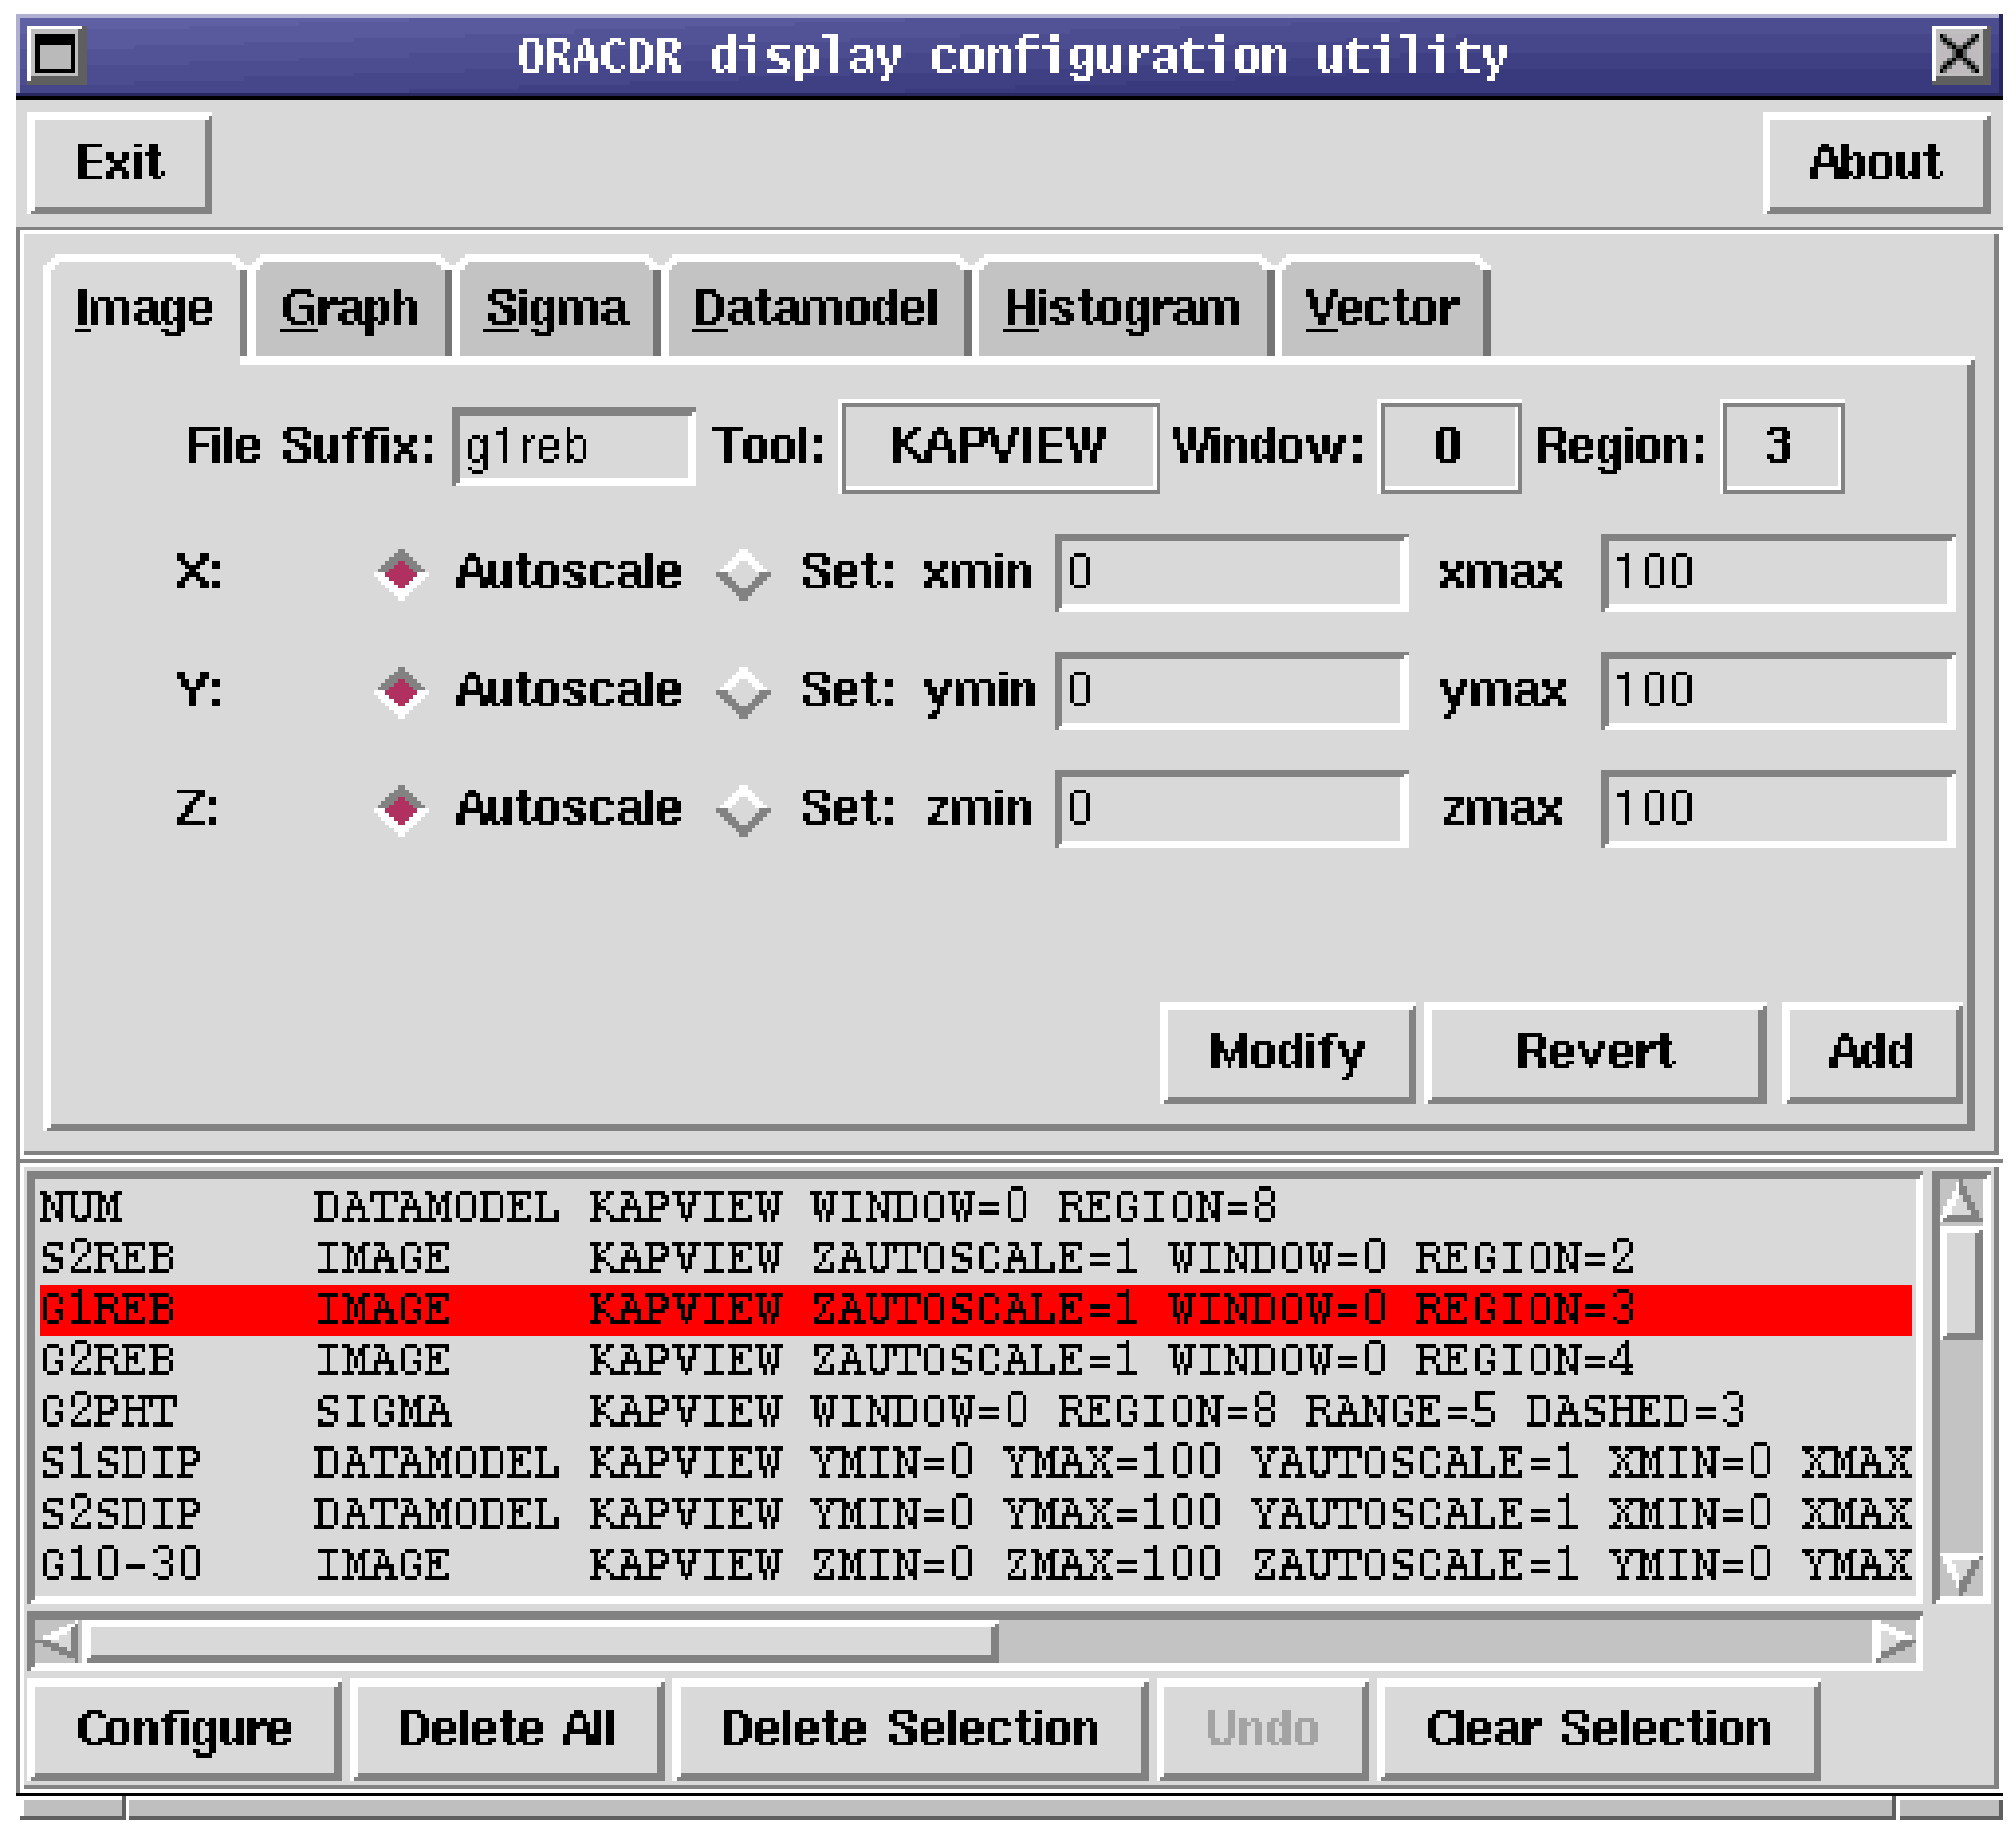
\includegraphics[width=\textwidth]{sun230_disp.eps}
\caption{The ORACDISP display configuration tool}
\end{figure}

\subsubsection*{How the pipeline displays\label{The_ORAC-DR_Display_System_How_the_pipeline_displays}\index{The ORAC-DR Display System!How the pipeline displays}}


The \emph{disp.dat} file has a series of entries consisting of a line
each. Each line has a series of space-separated items.  All but
the first item, the suffix, use the keyword=value syntax.



These items are:

\begin{description}

\item[{suffix}] \mbox{}

A file suffix representing a particular step of the data reduction
process as designated by that instrument's file naming convention. For
example, for UFTI data ``dk'' states what to do with a file called
 \texttt{f19990330\_00042\_dk.sdf}. Many entries may be made for a particular
suffix. The following special conventions are used: NUM describes a
file ending in just an observation number (usually representing raw
data). For instruments that have multiple data arrays in a single data
frame, S2$<$suffix$>$ (e.g. S2dk) represents the second data array in the
frame with the \_dk suffix.


\item[{tool}] \mbox{}

A display tool such as \texttt{Gaia} or \texttt{KAPVIEW} (the latter being a collective
term for various \texttt{KAPPA} display tasks). The tools available are
determined by the display type (q.v.) selected.


\item[{type}] \mbox{}

A display type such as graph, image, contour etc.  These vary according
to the tool selected.   The following types are available.  The tools
which support the given display type are listed in parentheses.

\begin{description}

\item[{contour (\texttt{KAPVIEW})}] \mbox{}

Plots a contour plot.


\item[{datamodel (\texttt{KAPVIEW})}] \mbox{}

Displays data (as points) with a model overlaid.


\item[{graph (\texttt{KAPVIEW}, \texttt{P4})}] \mbox{}

Plots a line graph such as a spectrum.


\item[{histogram (\texttt{KAPVIEW})}] \mbox{}

Plots a line graph such as a spectrum.


\item[{image (\texttt{GAIA}, \texttt{KAPVIEW},}] \textbf{\texttt{P4})}

Displays an image.


\item[{sigma (\texttt{KAPVIEW})}] \mbox{}

Draws a scatter plot with a Y range of +/- N standard deviations.


\item[{vector (\texttt{KAPVIEW})}] \mbox{}

Displays an image and vectors (e.g. polarimetry data).

\end{description}

\item[{region}] \mbox{}

For device tools that support it, region addresses the parts of a
window where a display ends up. For KAPVIEW, these are: whole screen
(0), top left quarter (1), top-right quarter (2), bottom-left quarter
(3), bottom-right quarter (4), left half (5), left right (6), top half
(7), bottom half (8).  Defaults to 0.


\item[{window}] \mbox{}

The number of the window in which the display is to go. The value of
this is simply an identifier and does not presuppose order. If you ask
for an image display to go to window 2 and you have configured no
displays to go to windows 0 and 1 then you will only get one window on
your screen. If you then configure a histogram display to go to window
2 it will go to the same window whereas if you configure it to go to
window 1 (or 5 or 9 or anything else besides 2) it will end up in its
own window. Note that no windows are launched until they are
required.


\item[{xautoscale}] \mbox{}

Specifies whether or not to use a section of the data frame.  If set to
1, meaning true, the whole X axis is used.  If set to 0, the pixel limits
are specified by keywords xmin and xmax.  The default is 1.



There are corresponding autoscaling keywords for higher dimensions
named yautoscale, 3autoscale, 4autoscale etc.


\item[{xmin, xmax}] \mbox{}

The X-axis pixel limits of the data to be displayed when xautoscale=1.
xmin should be less than or equal to xmax.  There are corresponding
pixel-range keywords for higher dimensions: ymin and ymax, 3min and
3max, 4min and 4max etc. when autoscaling on the corresponding axis is
disabled.


\item[{zautoscale}] \mbox{}

Set to 1 meaning true, this scales this requests that the data are
scaled automatically between the data range.  In the case of images on
GAIA the cut is at the 95 percentile.  When zautoscale is 0, the
scaling is between the limits defined by keywords zmin and zmax.
Defaults to 1 if absent.


\item[{zmin, zmax}] \mbox{}

When zautoscale is 1, these specifiy the lower and higher
scaling limits for the data values.


\item[{cut}] \mbox{}

If the number of dimensions in the data file is greater than that
requested, sections in higher dimensions are set to 1 by compressing
the undesired dimension(s).  Option cut specifies the desired
dimension(s).



Option cut is a comma-separated list specifying the dimensionality and
axes to retain.  The number of entries should equal the dimensionality
needed by the type of plot.  For instance, a graph only one value is
required since a graph is 1-D.  The allowed values are X, Y, 3, 4, or
5. If the number of dimensions in the data file is fewer than that
requested, ORAC-DR prints a warning message.



Here are two examples, a graph can be displayed from a 2-dimensional
image by displaying a cut in the X direction (averaging over the Ys)
by setting cut=X.   A `white-light' contour plot of a x,y,wavelength
spectral data cube may be plotted using cut=X,Y.

\end{description}


There are also parameters special to particular types of display,
which also use the keyword=value syntax.  These are:

\begin{description}

\item[{angrot}] \mbox{}

The angle to add to all vectors in a type=vector plot.


\item[{comp}] \mbox{}

The array component to display.  Allowed values are Data, Variance, or
Error.  The default is Data.  This applies to type=contour, datamodel,
graph, histogram, image, or sigma displays.


\item[{dashed}] \mbox{}

The location of the dashed lines for a type=sigma display in standard
deviaiton units.  This defaults to 3.


\item[{errbar}] \mbox{}

If set to 1 (true), error bars are plotted on a type=graph display,
provided there is variance information present.  The default is 0,
meaning do not plot error bars.


\item[{multivector}] \mbox{}

This controls the appearance of vectors in a type=vector plot.
If set to 0 (false), the default, the vectors are white and have
thickness 1.  If set to 1 (true), the vectors are yellow with a blue
trim and have thickness three.


\item[{nbins}] \mbox{}

This is the number of bins to be used for histogram calculation for
type=histogram.  It defaults to 20.


\item[{ncont}] \mbox{}

This specifies the number of contours to plot for type=contour.
It defaults to 6 if a non-positive value is supplied.


\item[{range}] \mbox{}

The standard-deviation range for a type=sigma display.  This defaults
to 5.


\item[{key}] \mbox{}

If set to 1 (true), a colour table key is drawn alongside the displayed
image. The default is 0, meaning no colour table key is drawn.

\end{description}
\subsubsection*{The order of play\label{The_ORAC-DR_Display_System_The_order_of_play}\index{The ORAC-DR Display System!The order of play}}


Every time a primitive creates a meaningful file with a particular
suffix, it sends a display request to the display system. For example,
suppose the primitive that performs dark subtraction creates a frame
called \texttt{f19990330\_00042\_dk.sdf} and then asks the display system to
display it. The display system consults the \emph{disp.dat} file for a dk
entry. If no such entry is found, the display request is ignored and
nothing happens. If one or more entries are found the display system
proceeds to honour the request. If the \emph{disp.dat} entry specifies a
particular tool and/or window, the display system checks to see if
they exist already and if not, stars them. Then it displays the data
with the appropriate parameters.

\subsection*{Document info\label{The_ORAC-DR_Display_System_Document_info}\index{The ORAC-DR Display System!Document info}}


Original author: frossie



\$Id\$


%% ORACDRDOC_HOWTO:Calibrating
\section{The ORAC-DR Calibration Selection\label{The_ORAC-DR_Calibration_Selection}\index{The ORAC-DR Calibration Selection}}


An ORAC-DR HOWTO

\subsubsection*{Description\label{The_ORAC-DR_Calibration_Selection_Description}\index{The ORAC-DR Calibration Selection!Description}}


ORAC-DR has a totally flexible system for controlling the automatic
selection of calibration frames.  This note describes how it works and
how to override it

\subsubsection*{What happens\label{The_ORAC-DR_Calibration_Selection_What_happens}\index{The ORAC-DR Calibration Selection!What happens}}


The type of calibrations used depend, obviously, on the instrument and
the data reduction recipes used. Typically there are three kinds of
calibration frames:

\begin{itemize}

\item

Library frames provided by the observatory (bad pixel masks, rotation
transformations, etc).  These are maintained by the instrument
scientist as appropriate.  They are located in \texttt{ORAC\_DATA\_CAL}.


\item

Nightly frames that are generated during observing.  The may be taken
in specific calibration observations, e.g. by taking a ``dark'' (at UKIRT)
or ``skydip'' (at JCMT) frames.  They might also be generated from
actual observations of targets (such as ``sky flats'') or
calibration values (such as ``flux conversion factors'') calculated
as part of a recipe.  These are located in \texttt{ORAC\_DATA\_OUT}.


\item

``Rule'' files that contain the rules for what constitutes an
appropriate calibration frame.  These are located in \texttt{ORAC\_DATA\_CAL}.

\end{itemize}


ORAC-DR treats the first two kinds rather differently.



Library frames reside \texttt{ORAC\_DATA\_CAL} and their selection is hardwired
either in the instrument class or in a DR primitive.  The users are
unlikely to be concerned with them unless they want to override them
with their own.



Nightly frames are handled in a more complicated way.  A DR recipe
that generates a calibration frame is responsible for filing it with
the pipeline.  The pipeline will hand it back to recipes that require
calibration recipes according to a set of rules that are defined on a
per-instrument basis by the ORAC-DR infrastructure as well as a
per-frame basis by the calibration rules files.

\subsubsection*{Finding calibration frames\label{The_ORAC-DR_Calibration_Selection_Finding_calibration_frames}\index{The ORAC-DR Calibration Selection!Finding calibration frames}}


When a frame is reduced and files as a calibration, it is added to an
index file located in \texttt{ORAC\_DATA\_OUT} named after the type of
calibration, e.g., dark frames are filed in \emph{index.dark}.  When the
pipeline is run up and needs a calibration frame but has not been
asked to reduce one in that session it will look in the index files
for one that may have been reduced at a previous time.



If the pipeline is unable to find a suitable calibration it will
complain vociferously and exit.  This may seem extreme, but remember
that ORAC-DR is designed for online use at an observatory.  If an
observer has not taken appropriate calibrations, we wish to point it
out to them in the strongest terms because we do not want them to end
up with un-reduceable data.

\subsubsection*{Overriding defaults\label{The_ORAC-DR_Calibration_Selection_Overriding_defaults}\index{The ORAC-DR Calibration Selection!Overriding defaults}}


You can override the pipeline's selection of calibration frame by
using the ORAC-DR \texttt{-calib} command line option.  Use this override
judiciously, as in general the pipeline does a fine job.



The ORAC-DR \texttt{-calib} command line option is used by giving comma
separated key=value pairs (e.g. '\texttt{-calib dark=file1,bias=file2}').
The following keys can be used for general instruments.  Specific
instruments may have extra calibration overrides that can be used.

\begin{itemize}

\item

baseshift - Use the given comma separated doublet (e.g. \texttt{"0,0"})
as the frame's base position.


\item

bias - Use the given frame as a bias.


\item

dark - Use the given frame as a dark.


\item

flat - Use the given frame as a flat.


\item

mask - Use the given frame as a mask. This option is usually used
for bad pixel masks.


\item

polrefang - Add the given value to the measured polarisation angle
to align the polarimeter's reference angle to north.


\item

readnoise - Use the given value for the detector readnoise.


\item

referenceoffset - Use the given comma separated doublet (e.g.
\texttt{"0,0"}) as the frame's reference offset, which is difference between
the frame centre and the reference pixel derived from the FITS
headers.


\item

rotation - Use the given frame as a rotation matrix.


\item

sky - Use the given frame as a sky observation.


\item

standard - Use the given frame as a standard star observation.

\end{itemize}


When files are given the extension should be left off.  As an example,
if you have made a new bad pixel mask and wish to use it with ORAC-DR,
the following command would be used:

\begin{verbatim}
 oracdr -calib mask=new_bpm
\end{verbatim}

%% ORACDRDOC_HOWTO:ShellVariables
\section{Shell Variables\label{Shell_Variables}\index{Shell Variables}}


An ORAC-DR HOWTO

\subsubsection*{Description\label{Shell_Variables_Description}\index{Shell Variables!Description}}


This document describes the complete list of environment variables
used by the pipeline.

\subsection*{Complete variable list\label{Shell_Variables_Complete_variable_list}\index{Shell Variables!Complete variable list}}


ORAC-DR uses a number of environment variables for configuration.

\subsubsection*{User variables\label{Shell_Variables_User_variables}\index{Shell Variables!User variables}}


Users may need to change the following variables before using the
software.

\begin{description}

\item[{\texttt{ORAC\_DATA\_ROOT}}] \mbox{}

Location of the raw and reduced data directories if it confirms with
the naming convention for the instrument. Should be set before the
instrument startup script, which uses this variable to set
\texttt{ORAC\_DATA\_IN} and \texttt{ORAC\_DATA\_OUT}.


\item[{\texttt{ORAC\_DATA\_IN}}] \mbox{}

Actual location of raw data files. Should be set after the instrument
startup script.


\item[{\texttt{ORAC\_DATA\_OUT}}] \mbox{}

Actual location of reduced data files. This is also the working
directory of the pipeline. Should be set after the instrument startup
script.


\item[{\texttt{ORAC\_CAL\_ROOT}}] \mbox{}

Directory where the instrument specific


\item[{\texttt{ORAC\_DATA\_CAL}}] \mbox{}

Location of the calibration files for the instrument. Set by the
instrument startup script to \texttt{ORAC\_CAL\_ROOT/$<$instrument$>$}.


\item[{\texttt{ORAC\_RECIPE\_DIR}}] \mbox{}

Location of user-defined recipes. These supersede any identically
names ones in \texttt{ORAC\_DIR/recipes/$<$instrument$>$}.


\item[{\texttt{ORAC\_PRIMITIVE\_DIR}}] \mbox{}

Location of user-defined primitives. These supersede any identically
names ones in \texttt{ORAC\_DIR/primitives/$<$instrument$>$}.


\item[{\texttt{ORACDR\_TMP}}] \mbox{}

Location of scratch files for the ADAM messaging system. If this
environment variable is not set, then this location will default to
\texttt{ORAC\_DATA\_OUT}.


\item[{\texttt{ORAC\_NOGROUPS}}] \mbox{}

If set, group processing will be disabled.


\item[{\texttt{ORAC\_KEEP}}] \mbox{}

If set, all intermediate files created by ORAC-DR will be kept.
This does not include temporary files; to keep temporary files
run ORAC-DR with the \texttt{-debug} flag.


\item[{\texttt{ORACDR\_PROXY}}] \mbox{}

If set, ORAC-DR will use a proxy for network lookups. This variable
should be set to the full proxy name, including the protocol, name,
and port. An example of this is "http://proxy.example.com:8181".

\end{description}
\subsubsection*{System variables\label{Shell_Variables_System_variables}\index{Shell Variables!System variables}}


Starlink and JAC users should not redefine these variables under
normal circumstances because they are correctly set by their user
logins. They are included here for reference only.

\begin{description}

\item[{\texttt{ORAC\_DIR}}] \mbox{}

The location of the ORAC-DR software directory. This is normally set
by a login script.


\item[{\texttt{ORAC\_INSTRUMENT}}] \mbox{}

The instrument under whose environment ORAC-DR should run. Normally
this is set by the appropriate instrument script in \texttt{ORAC\_DIR/etc/}


\item[{\texttt{ORAC\_PERL5LIB}}] \mbox{}

The location of the ORAC-DR perl libraries. These are normally in
\texttt{ORAC\_DIR/lib/perl5}.


\item[{\texttt{ORAC\_PERSON}}] \mbox{}

The e-mail address of the person who supports ORAC-DR for
\texttt{\$ORAC\_INSTRUMENT}. This is used in the splash screen.
(This was formerly the JAC contact name and assumed a JAC
e-mail address \texttt{\$ORAC\_PERSON@jach.hawaii.edu}.)


\item[{\texttt{ORAC\_LOOP}}] \mbox{}

The default type of looping scheme that should be used for online
reduction of \texttt{ORAC\_INSTRUMENT}. This  is used in the splash screen.


\item[{\texttt{ORAC\_SUN}}] \mbox{}

The Starlink User Note number that documents the data reduction for
\texttt{ORAC\_INSTRUMENT}. This  is used in the splash screen.

\end{description}
\subsection*{Document info\label{Shell_Variables_Document_info}\index{Shell Variables!Document info}}


Original author: frossie



\$Id\$


%% ORACDRDOC_BIN:oracdisp
\section{oracdisp\label{oracdisp}\index{oracdisp}}


Control ORAC-DR display environment

\subsection*{SYNOPSIS\label{oracdisp_SYNOPSIS}\index{oracdisp!SYNOPSIS}}
\begin{verbatim}
  oracdisp [-h] [-v] [-in=file] [-out=file]
\end{verbatim}
\subsection*{DESCRIPTION\label{oracdisp_DESCRIPTION}\index{oracdisp!DESCRIPTION}}


Controls the display environment used by ORAC-DR. This routine
can be used to edit the current environment and add display directives
to the current environment.

\subsection*{ARGUMENTS\label{oracdisp_ARGUMENTS}\index{oracdisp!ARGUMENTS}}


The following command line arguments are recognised by \texttt{oracdisp}:

\begin{description}

\item[{\textbf{-h}}] \mbox{}

Prints help information describing the arguments.


\item[{\textbf{-v}}] \mbox{}

Prints version number information.


\item[{\textbf{-in}}] \mbox{}

Used to modify the name of the input display definition file.
Default is \emph{disp.dat}. Do not modify if used in conjunction with
ORAC-DR.


\item[{\textbf{-out}}] \mbox{}

Used to modify the name of the output display definition file.
Default is \emph{disp.dat}. Do not modify if used in conjunction with
ORAC-DR.

\end{description}
\subsection*{NOTES\label{oracdisp_NOTES}\index{oracdisp!NOTES}}


By default, \texttt{oracdisp} manipulates a file called \emph{disp.dat}
in the \texttt{ORAC\_DATA\_OUT} directory. Do not modify the name of this
file for use with ORAC-DR (since ORAC-DR is expecting a file
called \emph{disp.dat} in \texttt{ORAC\_DATA\_OUT}).



If \texttt{ORAC\_DATA\_OUT} is not set, and no overrides provided on the
command-line, the program will try to find \emph{disp.dat} in the current
directory.

\subsection*{AUTHORS\label{oracdisp_AUTHORS}\index{oracdisp!AUTHORS}}


Tim Jenness (t.jenness@jach.hawaii.edu),
Frossie Economou (frossie@jach.hawaii.edu)

\subsection*{SEE ALSO\label{oracdisp_SEE_ALSO}\index{oracdisp!SEE ALSO}}


\emph{oracdr}

\subsection*{REVISION\label{oracdisp_REVISION}\index{oracdisp!REVISION}}


\$Id\$

\subsection*{COPYRIGHT\label{oracdisp_COPYRIGHT}\index{oracdisp!COPYRIGHT}}


Copyright (C) 1998-2000 Particle Physics and Astronomy Research
Council. All Rights Reserved.


%% ORACDRDOC_BIN:oracdr_nuke
\section{oracdr\_nuke\label{oracdr_nuke}\index{oracdr\ nuke}}


Kill all ORAC-DR related processes and shared memory

\subsection*{SYNOPSIS\label{oracdr_nuke_SYNOPSIS}\index{oracdr nuke!SYNOPSIS}}
\begin{verbatim}
  oracdr_nuke
\end{verbatim}
\subsection*{DESCRIPTION\label{oracdr_nuke_DESCRIPTION}\index{oracdr nuke!DESCRIPTION}}


Attempt to kill all ORAC-DR related processes and shared memory that
can be found and that are associated with the current user.

\subsection*{NOTES\label{oracdr_nuke_NOTES}\index{oracdr nuke!NOTES}}
\begin{itemize}

\item

All shared memory owned by the current user is removed even if
it is not directly associated with an ORAC-DR process.


\item

Will not attempt to remove shared memory owned by another user.


\item

Will attempt to kill processes owned by other users even though
this will not succeed unless the user has special privilege.


\item

Does not attempt to clear out ADAM\_USER directories. This is not
normally a problem for ORAC-DR since each ORAC-DR process works
in a different ADAM\_USER directory.


\item 

Takes an optional \texttt{-nogaia} option. If this option is present on the
command line, then GAIA processes will not be killed.

\end{itemize}
\subsection*{AUTHORS\label{oracdr_nuke_AUTHORS}\index{oracdr nuke!AUTHORS}}


Frossie Economou (frossie@jach.hawaii.edu),
Tim Jenness (t.jenness@jach.hawaii.edu),
Alasdair Allan (aa@astro.ex.ac.uk),
Brad Cavanagh (b.cavanagh@jach.hawaii.edu)

\subsection*{REVISION\label{oracdr_nuke_REVISION}\index{oracdr nuke!REVISION}}


\$Id\$

\subsection*{COPYRIGHT\label{oracdr_nuke_COPYRIGHT}\index{oracdr nuke!COPYRIGHT}}


Copyright (C) 1996-2006 Particle Physics and Astronomy Research Council.
All Rights Reserved.




% ? End of main text
\end{document}
